
\section{RNN based model Evaluation}\label{sec:rnneval}
From the graphs shown in Figure~\ref{fig:grruntraining},
we can see that the training phase was successful,
and after an initial descent, the loss values remained relatively
constant without displaying any abnormal trends.
The statistics presented in Figure~\ref{fig:grrunsysusage} reveal
that the machine at our disposal was not fully utilized,
suggesting that this architecture can be trained and used on
less powerful computers than the one we have.
Additionally, the model appears to be very lightweight, both in terms
of the relatively small number of parameters and its weight,
which doesn't exceed 400~KB. The inference time does not even
approach one second, making it extremely fast in execution.

\begin{table}[H]
	\begin{center}
		\begin{tabular}[c]{l|l|l|l}
			%\cline{2-4}
			\multicolumn{1}{c|}{\textbf{Gap Period}} &
			\multicolumn{1}{c|}{\textbf{MAE (kW)}}   &
			\multicolumn{1}{c|}{\textbf{MAPE (\%)}}  &
			\multicolumn{1}{c}{\textbf{R}$^2$}                             \\
			\hline

			02-04 to 05-04                           & 4.72 & 28.12 & 0.96 \\
			03-04 to 06-04                           & 5.11 & 33.01 & 0.91 \\
			04-04 to 04-04                           & 3.60 & 27.15 & 0.93 \\
			07-03 to 10-4                            & 7.52 & 34.22 & 0.90 \\
			12-04 to 14-04                           & 6.61 & 20.68 & 0.96
			% 06-04 to 07-04 & 20.07 & 0.62 &1293.53&50.70&1293.53&25.22 \\
		\end{tabular}
	\end{center}
	\caption{The table displays the MAE, MAPE, and R$^2$ values applied to some model predictions during the testing phase, some of which are shown in Figure~\ref{fig:grrunevalplots}.
	}\label{tab:grrunpmaer}
	%La tabella mostra i valori del MAE, MAPE e dell'indice R$^2$ applicate ad alcune predizioni del modello durante la fase di testing, alcune delle quali sono mostrate nella Figura~\ref{}.}\label{tab:dfsplit}
\end{table}


\begin{table}[H]
	\centering
	\begin{tabular}{l|l|l|l}
		                                        &
		\multicolumn{1}{c|}{\textbf{MAE (kW)}}  &
		\multicolumn{1}{c|}{\textbf{MAPE (\%)}} &
		\multicolumn{1}{c}{\textbf{R$^2$}}                            \\
		\hline
		\textbf{AVG}                            & 6.92 & 30.32 & 0.92 \\
		\textbf{STD. DEV}                       & 1.74 & 9.30  & 0.05
	\end{tabular}
	\caption{Global metrics for the RNN-based model calculated on gaps of varying sizes.}
	\label{tab:grrunglobalmetrics}
\end{table}


%\begin{table}[H]
%\begin{minipage}[t]{.45\textwidth}
%	\begin{center}
%		\begin{tabular}[c]{l|l|l}
%            \multicolumn{3}{c}{\textbf{\textit{02-04 to 05-04 Gap}}} \\
%			%\hline
%            & \multicolumn{1}{c|}{\textbf{MAE (kW)}} &
%            \multicolumn{1}{c}{\textbf{MAPE (\%)}} \\
%            \hline          
%            \textbf{Day 1} & 97.03 &	1.99 \\
%            \textbf{Day 2} & 28.68 &	3.22 \\
%            \textbf{Day 3} & 69.79 &	4.79 \\
%            \textbf{Day 4} & 41.65 &    1.98
%		\end{tabular}
%  %\caption{}
%	\end{center}
%\end{minipage}%
%\hfill
%\begin{minipage}[t]{.45\textwidth}
%	\begin{center}
%		\begin{tabular}[c]{l|l|l}
%            \multicolumn{3}{c}{\textbf{\textit{12-04 to 14-04 Gap}}} \\
%			%\hline
%            & \multicolumn{1}{c|}{\textbf{MAE (kW)}} &
%            \multicolumn{1}{c}{\textbf{MAPE (\%)}} \\
%            \hline          
%            \textbf{Day 1}& 151.93 &	2.86 \\
%            \textbf{Day 2} &49.44 & 1.01\\
%            \textbf{Day 3} &111.25 &	2.76
%		\end{tabular}
%        %\caption{}
%	\end{center}
%\end{minipage}%
%\vspace{.5cm}
%\begin{minipage}{\textwidth}
%	\begin{center}
%		\begin{tabular}[c]{l|l|l}
%            \multicolumn{3}{c}{\textbf{\textit{04-04 to 04-04 Gap}}} \\
%			%\hline
%            & \multicolumn{1}{c|}{\textbf{MAE (kW)}} &
%            \multicolumn{1}{c}{\textbf{MAPE (\%)}} \\
%            \hline          
%            \textbf{Day 1} & 0.93 &	0.06
%		\end{tabular}
%  %\caption{}
%	\end{center}
%\end{minipage}
%\caption{The tables display the Daily MAE\cite{metrics} and MAPE\cite{metrics} values related to the graphs shown in Figure~\ref{fig:grrunevalplots}.}\label{tab:grrundailymetrics}
%%Nelle tabelle sono mostrati i valori giornalieri di MAE e MAPE relativi ai grafici mostrati in Figura~\ref{fig:grrunevalplots}.}
%\end{table}

%Dai grafici mostrati in Figura~\ref{fig:grruntraining} possiamo vedere come la fase di addestramento
%è andata a buon fine e, dopo una parte iniziale di discesa, i valori delle loss sono rimasti pressochè costanti e non mostrano andamenti anomali. Dalle statistiche riportate in Figura~\ref{fig:grrunsysusage} possiamo vedere come la macchina a nostra disposizione non è
%stata sfruttata a pieno e questo può portarci a pensare che questa architettura sia allenabile ed
%utilizzabile su computer meno perfromanti di quello a nostra disposizione. Inoltre il modello 
%risulta essere molto leggero, sia per il numero relativamente ridotto di parametri sia per il 
%peso che non supera i 400 KB.

\begin{figure}[H]
	\centering
	\begin{subfigure}{\textwidth}
		\centering
		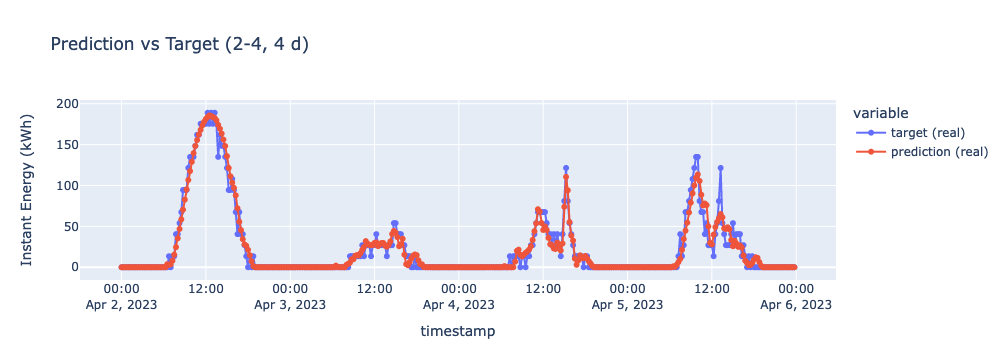
\includegraphics[width=\textwidth]{chapters/3_models/imgs/grrun/eval/grruneval24.png}
		\caption{}
	\end{subfigure}
	\begin{subfigure}{\textwidth}
		\centering
		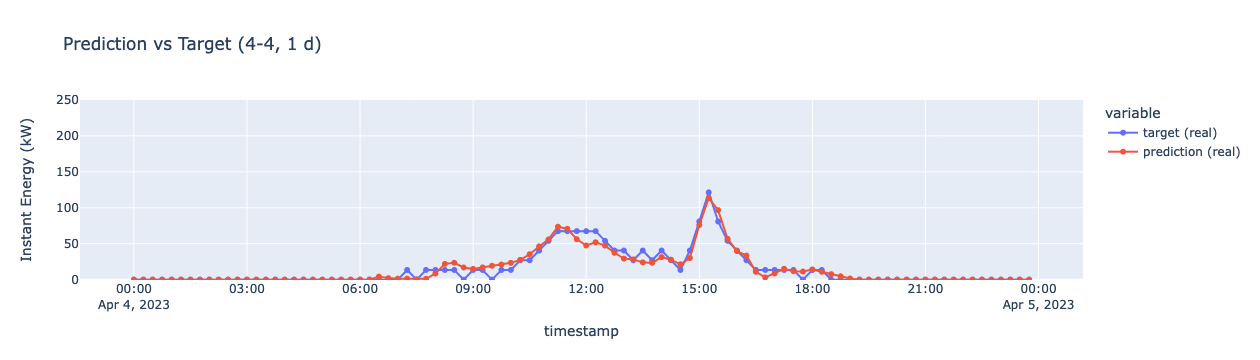
\includegraphics[width=\textwidth]{chapters/3_models/imgs/grrun/eval/grruneval44.png}
		\caption{}
	\end{subfigure}
	\begin{subfigure}{\textwidth}
		\centering
		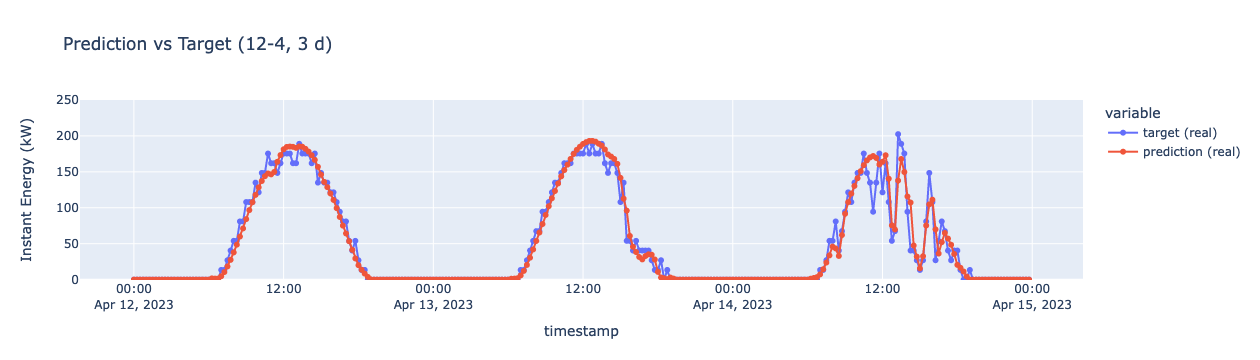
\includegraphics[width=\textwidth]{chapters/3_models/imgs/grrun/eval/grruneval124.png}
		\caption{}
	\end{subfigure}
	\caption{In the figure, three model predictions (in red) are shown alongside the ground truth (in blue) for gaps of varying sizes. These predictions were made using data from the testing dataset. The tensors \textit{before}, \textit{after}, and \textit{future} have variable dimensions, as described earlier.}
	%In figura vengono mostrate 3 predizioni del modello (in rosso) comparate con la ground thorught (in blu) di buchi a dimensione variabile. Queste predizioni sono state effettuate con i dati provenienti dal dataset di Testing.}
	\label{fig:grrunevalplots}
\end{figure}
\newpage
Analyzing some model predictions as shown in
Figure~\ref{fig:grrunevalplots}, we can observe how the real
instant energy production curves (displayed in blue) are
closely approximated by the model (red curves).
The model effectively understands the plant's behavior,
even managing to predict production spikes.
We can also see that energy production is consistently zero during
the night, and it adeptly captures the
day/night cycle by gradually reducing production as sunset approaches.

In graph (a), we can see a 4-day gap from 02-04-2023 to 06-04-2023.
The first two days are predicted very well, while in the last part,
we can see that a production spike was not detected.
For this period we have a quite high $R^2$ index of 0.96, 4.72 kW as MAE and 28.12 \%  for the MAPE, which are quite good values.
In graph (b), we can observe a 1-day gap on 04-04-2023. We notice that the overall trend is almost entirely approximated correctly, except for some time intervals around 12:00, indeed, we have slightly better results with an MAE of 3.60 kW and a MAPE of 27.15\%.
The last graph (c) is related to a 3-day gap, and we can see that the first two days are approximated well, while in the last day, the production spikes are identified but with values not entirely similar to those of the ground truth.
All the results presented so far are consistent with the average values shown in Table~\ref{tab:grrunglobalmetrics} demonstrating that the model returns fairly consistent outputs among them.
%Analizzando alcune predizioni del modello riportate in Figura~\ref{fig:grrunevalplots} possiamo notare come le curve dell'energia 
%istantanea prodotta realmente (mostrate in blu) vengono approssimate decisamente
%bene dal modello (curve in rosso). Il modello riesce a capire bene il comportamento
%dell'impianto riuscendo anche a prevedere eventuali picchi di produzione.
%Possiamo notare come di notte la produzione di energia nelle predizioni è sempre nulla e come riesce molto bene a comprendere il ciclo giorno/notte
%andando ad azzerare gradualmente la produzione quando si avvicina il tramonto.

%Nel grafico (a) possiamo vedere un buco di 4 giorni che va dal 02-04-2023 al 06-04-2023. I primi due giorni vengono predetti molto bene, mentre nell'ultimo possiamo vedere che un picco di produzione non è stato individuato.
%Nel prolt (b) possiamo apprezzare un buco di 1 giorno, il 04-04-2023.
%Notiamo come l'andamento è quasi del tutto approsiamoto correttamente tranne
%che per alcuni intervalli temporali che si aggirano intorno le 12:00.
%L'ultimo grafico (c) è relativo ad un buco di 3 giorni e possiamo vedere
%come i primi due vengono approssimati bene, mentre nell'ultimo i picchi
%di produzione vengono si individuati ma con valori non del tutto simili
%a quelli della ground truth.

\begin{figure}[H]
	\centering
	\begin{subfigure}{\textwidth}
		\centering
		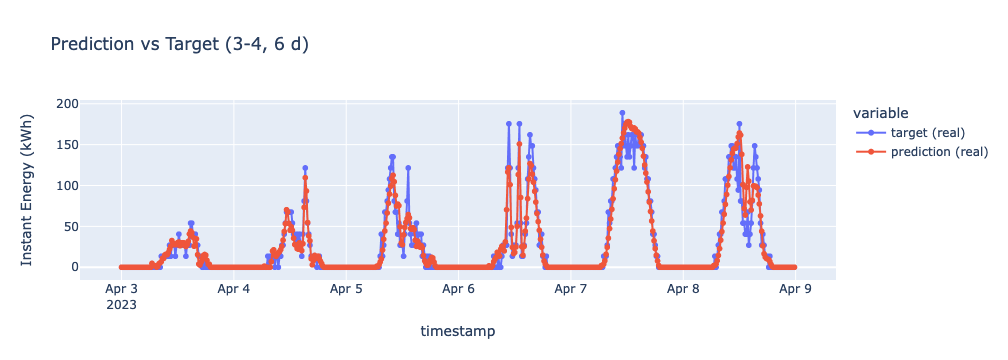
\includegraphics[width=.85\textwidth]{chapters/3_models/imgs/grrun/eval/grruneval6buco.png}
		\caption{}
	\end{subfigure}
	\begin{subfigure}{\textwidth}
		\centering
		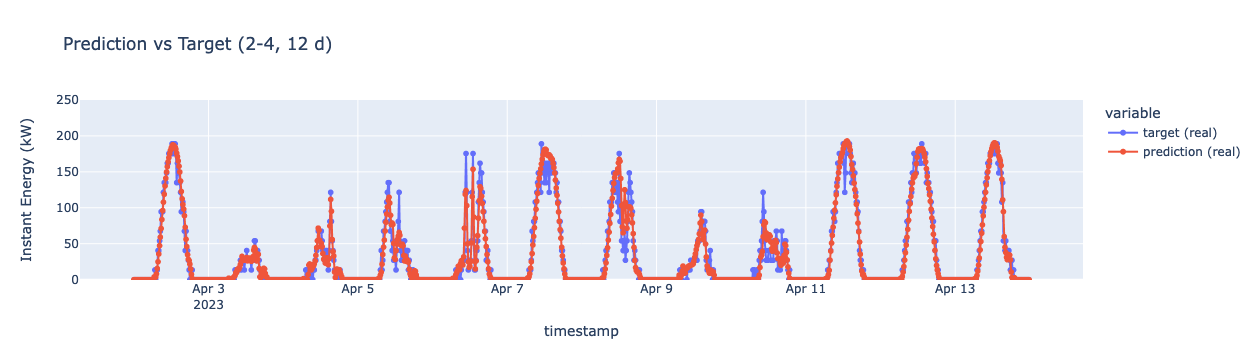
\includegraphics[width=.85\textwidth]{chapters/3_models/imgs/grrun/eval/grruneval12buco.png}
		\caption{}
	\end{subfigure}
	\caption{The graphs depict two model predictions for gaps that exceed the maximum limit of days set during the training phase. The first one (a) shows a 6-day gap, while the second one (b) presents a 12-day gap.}
	%I grafici mostrano due predizioni del modello di buchi con dimensioni che superano il limite massimo di giorni impostati nella fase di training. Il primo (a) mostra un buco di 6 giorni, mentre il secondo (b) uno di 12.}
	\label{fig:grrunevalbucogrande}
\end{figure}

It is interesting to note how the model still performs well even
when presented with gaps that exceed the maximum length set
during training.
In Figure~\ref{fig:grrunevalbucogrande}, two graphs are shown:
(a) represents a 6-day gap (two days longer than the training length),
and (b) a 12-day gap (eight days longer than the training length).

\begin{table}[H]
	\begin{center}
		\begin{tabular}[c]{l|l|l|l}
			%\cline{2-4}
			\multicolumn{1}{c|}{\textbf{Gap Period}} &
			\multicolumn{1}{c|}{\textbf{MAE (kW)}}   &
			\multicolumn{1}{c|}{\textbf{MAPE (\%)}}  &
			\multicolumn{1}{c}{\textbf{R}$^2$}                             \\
			\hline

			03-04 to 08-04                           & 6.56 & 30.94 & 0.92 \\
			02-04 to 13-04                           & 5.99 & 27.50 & 0.95

			% 06-04 to 07-04 & 20.07 & 0.62 &1293.53&50.70&1293.53&25.22 \\
		\end{tabular}
	\end{center}
	\caption{The table displays the MAE, MAPE, and R$^2$ values applied to the model predictions shown in Figure~\ref{fig:grrunevalbucogrande}.
	}\label{tab:grrunpmaerlungo}
	%La tabella mostra i valori del MAE, MAPE e dell'indice R$^2$ applicate ad alcune predizioni del modello durante la fase di testing, alcune delle quali sono mostrate nella Figura~\ref{}.}\label{tab:dfsplit}
\end{table}


\begin{table}[H]
	\centering
	\begin{tabular}{l|l|l|l}
		\multicolumn{1}{c|}{\textbf{Gap Size}}      &
		\multicolumn{1}{c|}{\textbf{AVG MAE (kW)}}  &
		\multicolumn{1}{c|}{\textbf{AVG MAPE (\%)}} &
		\multicolumn{1}{c}{\textbf{AVG R$^2$}}                                                              \\
		\hline
		\textbf{12 days}                            & 6.64 $\pm$ 0.79 & 25.66 $\pm$ 5.90  & 0.95 $\pm$ 0.02 \\
		\textbf{\ 6 days}                           & 6.85 $\pm$ 0.93 & 27.44  $\pm$ 6.78 & 0.94 $\pm$ 0.02 \\
		\textbf{\ 2 days}                           & 6.86 $\pm$ 1.87 & 28.83 $\pm$ 10.02 & 0.92 $\pm$ 0.06 \\
		\textbf{< 60 ts}                            & 8.93 $\pm$ 2.22 & 36.14 $\pm$ 4.40  & 0.86 $\pm$ 0.07
	\end{tabular}
	\caption{Global results for the RNN-based model with fixed gap size. The table provides the average values along with their respective standard deviations.}
	\label{tab:grrunglobalmetricsranging}
\end{table}




%Given these results, we can conclude that the model can
%generalize effectively and predict instant energy production
%trends with considerable reliability.


%\'{E} interessante notare come il modello riesce a perforare comunque bene anche se gli vengono passati dei buchi che superano la dimensione massima impostata durante l'addestramento. In Figura~\ref{fig:grrunevalbucogrande} vengono mostrati due grafici, (a) è un buco di 6 giorni (due in più della dimensione massima), mentre (b) è di 12. Dati questi risultati possiamo
%affermare che il modello è in grado di generalizzare molto bene e riuscire
%a predirre l'andamento dell'energia istantanea prodotta con notevole affidabilità.

%\begin{table}[H]
%\begin{minipage}[t]{.45\textwidth}
%	\begin{center}
%		\begin{tabular}[t]{l|l|l}
%            \multicolumn{3}{c}{\textbf{\textit{03-04 to 08-04 Gap}}} \\
%			%\hline
%            &
%            \makecell{\textbf{MAE}\\\textbf{(kW)}} &
%            \makecell{\textbf{MAPE}\\\textbf{(\%)}} \\
%            %\multicolumn{1}{c|}{\textbf{MAE (kW)}} &
%            %\multicolumn{1}{c}{\textbf{MAPE (\%)}} \\
%            \hline          
%            \textbf{Day 1}& 56.76 &	6.37 \\
%            \textbf{Day 2} &82.02 &	5.63\\
%            \textbf{Day 3} &59.90 &	2.84\\
%            \textbf{Day 4} & 150.79 &	5.91\\
%            \textbf{Day 5} & 12.52 &	0.24\\
%            \textbf{Day 6} & 238.88 &	6.73
%		\end{tabular}
%        %\caption{}
%	\end{center}
%\end{minipage}%
%\hfill
%\begin{minipage}[t]{.45\textwidth}
%	\begin{center}
%		\begin{tabular}[t]{l|l|l}
%            \multicolumn{3}{c}{\textbf{\textit{02-04 to 13-04 Gap}}} \\
%			%\hline
%            & 
%            \makecell{\textbf{MAE}\\\textbf{(kW)}} &
%            \makecell{\textbf{MAPE}\\\textbf{(\%)}} \\
%            %\multicolumn{1}{c|}{\textbf{MAE (kW)}} &
%            %\multicolumn{1}{c}{\textbf{MAPE (\%)}} \\
%            \hline          
%            \textbf{Day 1} & 148.45 &	3.04\\
%            \textbf{Day 2} & 38.14 &	4.28\\
%            \textbf{Day 3} & 55.41 &	3.80\\
%            \textbf{Day 4} & 20.26 &	0.96\\
%            \textbf{Day 5} & 104.28 &	4.09\\
%            \textbf{Day 6} & 112.09 &	2.18\\
%            \textbf{Day 7} & 312.26 &	8.79\\
%            \textbf{Day 8} & 47.65 &	3.46\\
%            \textbf{Day 9} & 16.32 &	0.99\\
%            \textbf{Day 10} & 23.08 &	0.43\\
%            \textbf{Day 11} & 240.66 &	4.52\\
%            \textbf{Day 12} & 22.21 &	0.45
%		\end{tabular}
%  %\caption{}
%	\end{center}
%\end{minipage}
%\caption{The tables presented refer to the graphs in Figure~\ref{fig:grrunevalbucogrande} and display the corresponding Daily MAE and MAPE metrics.}\label{tab:grrunbuchigrandi}
%%Le tabelle mostrate fanno riferimento ai grafici in Figura~\ref{fig:grrunevalbucogrande} e mostrano le relative metriche Daily MAE e MAPE.}
%%Nelle tabelle sono mostrati i valori giornalieri di MAE e MAPE relativi ai grafici mostrati in Figura~\ref{fig:grrunevalplots}.}
%\end{table}

Taking into account the data in Tables~\ref{tab:grrunpmaer},\ref{tab:grrunglobalmetrics},\ref{tab:grrunpmaerlungo} and \ref{tab:grrunglobalmetricsranging}, it can be confirmed that this
Recurrent Neural Network-based model is highly performant.
The average MAE value is 6.92 kW$\pm 1.74$, which is relatively low, while the average $R^2$ index is 0.92$\pm 0.05$, and it almost always approaches the ideal value of 1.0\cite{metrics}. Furthermore, the average MAPE value is 30.32$\pm 9.30$, which is a significant improvement compared to the previous model.

%The average MAE value is 6.92 kW $\pm 1.74$, that is consistently remains low, not exceeding 10 kW,
%while the $R^2$ index almost always approaches the ideal value of 1.0\cite{metrics}, never dropping below 0.70 (a value reached only in rare cases). Furthermore, the Daily MAPE values barely exceed 6\%, indicating very low daily error. The Global MAPE is 3.17\%, and the Global MAE is 95.75 kW, demonstrating excellent overall performance.

Equally positive results are obtained for gaps that exceed the
maximum training phase length of 4 days.
From Table~\ref{tab:grrunglobalmetricsranging}, we can see that for the
12, 6 and 2-day gaps, the average MAE, MAPE and $R^2$ index are quite similar compared to the values shown in Table~\ref{tab:grrunglobalmetrics},
some are slightly better, while others are slightly worse, but they remain stable and confirm the values shown earlier.
Clearly, we see a drop in performance with gap sizes shorter than 60 timestamps, as evident from the increase in MAE and MAPE and the decrease in the $R^2$ index.

%never exceeds 9\%, occasionally even reaching as low as 0.45\% error. The largest error is found on day 7, with a value of 312.26 kW.
%Similarly, for the 6-day gap, the MAPE values do not exceed 10\%,
%and the maximum error is found on the last day, with around
%239 kW (6.73\%).
%For both graphs, we have an $R^2$ value greater than 0.90, specifically 0.92 and 0.97, with a Gap MAE of 6.56 and 6.37 kW.

In conclusion, it can be affirmed that this model effectively
harnesses the potential offered by Recurrent Neural Networks and
excels in predicting the trend of instant energy production
during data gaps, even for gaps spanning multiple days.
%Prendendo in esame le Tabelle~\ref{tab:grrunpmaer} e \ref{tab:grrundailymetrics} possiamo confermare che questo modello basato
%su Recurrent Neaural Network sia molto performante. Vediamo come
%il \textit{Gap MAE} riamnga sempre basso, non superando i 10 kW, mentre 
%l'indice $R^2$ si avvicini quasi sempre al valore ideale di 1.0\cite{metrics} e comunque non scendendo mai sotto a 0.70 (valore raggiunto solo in rarissimi casi).
%Inoltre i valori del Daily MAPE superano a malapena il 6\% indicando un
%bassissimo errore giornaliero che globalmente risulta essere di 3.17\% per 
%il \textit{Global MAPE} e di 95.75 kW per il \textit{Global~MAE}.

%Altrettanto positivi sono i dati dei buchi che eccedono la dimensione massima di 4 giorni. Dalla Tabella~\ref{tab:grrunbuchigrandi}
%possiamo vedere che per il buco di 12 giorni il Daily MAPE non supera mai
%il 9\% raggungendo alle volte anche il 0.45\% di errore. L'errore più grande
%è relativo al giorno 7 per un valore di 312.26 kW.
%Similmente per il buco da 6 giorni abbiamo valori del MAPE che non superano
%il 10\% e l'errore massimo lo troviamo nell'ultimo giorno con circa 239 kW (6.73\%). Per tutti e due i grafici abbiamo un valore dell'indice $R^2$ superiore
%al .90, relativamente 0.92 e 0.97 con un Gap MAE di 6.56 e 6.37 kW.

%In conclusione possiamo affermare che questo modello riesce a sfruttare a pieno
%le potenzialità offerte dalle Reti Ricorrenti e riesce notevolmente bene
%a predirre l'andamento dell'energia istantanea prodotta durante bunchi di
%dati anche di molteplici giorni.